% Plantilla del curso: reemplazar el preámbulo por el .tex oficial descargado del enlace del enunciado
% y conservar los \input de las secciones.
\documentclass[10pt,twocolumn]{article}
\usepackage[utf8]{inputenc}
\usepackage[spanish]{babel}
\usepackage{amsmath,amssymb,graphicx,booktabs,algorithm,algpseudocode,natbib,hyperref}
\usepackage[margin=2cm]{geometry}
\graphicspath{{../results/figures/}}

\title{Clasificación ordinal bayesiana del nivel de riesgo materno a partir de variables fisiológicas}
\author{Sara Gabriela Chisaba Cárdenas, Alejandra Cortes Murillo, Juan Esteban Silva Arévalo\\
Pregrado Ciencia de Datos, Universidad Externado de Colombia}
\date{Entrega: xx de noviembre de 2026}

\begin{document}
\maketitle
% Responsable: A
\begin{abstract}
\textbf{Resumen.} % TODO
\textbf{Palabras clave:} % TODO
\end{abstract}
% TODO: Abstract y Keywords en inglés.
        % A
% Responsable: A
\section{Introducción}
\subsection{Contexto}

La reducción de la mortalidad materna y fetal, junto con tratamientos oportunos
durante el embarazo son factores prioritarios a nivel de sanidad pública global
lo cual se alinea con los ODS, como se menciona en ONU Mujeres ``\emph{Meta 3.1
de los ODS: Reducir la tasa mundial de mortalidad materna a menos de 70 por cada
100\,000 nacidos vivos\ldots Un poco más del 90\,\% de todas las muertes maternas
ocurren en países de ingresos y medios bajos en 2023}''. Por eso el principal
problema radica en situaciones de monitorización primaria en zonas rurales o
vulnerables de un país en desarrollo junto con la identificación temprana de los
síntomas y/o complicaciones para descubrir el nivel de riesgo en función del
seguimiento continuo de signos vitales como la frecuencia cardíaca, presión
arterial sistólica, temperatura corporal, entre otras. Sin embargo, evaluaciones
puntuales o un control inconsistente dificultan la detección a tiempo de
condiciones médicas que afectan tanto a la madre como al bebé y la Organización
Mundial de la Salud [OMS] (2025) indica que \emph{la mayoría de las muertes
maternas son prevenibles, ya que existen soluciones sanitarias bien conocidas
para prevenir o controlar las complicaciones}.

No obstante, se depende demasiado del presupuesto público y gubernamental para el
financiamiento de proyectos de tecnologías o nuevas infraestructuras en la salud
pública (Ramos Vázquez, 2019), ``\emph{La mayoría de muertes, lesiones y
problemas de salud se pueden evitar mejorando el acceso a servicios adecuados de
atención de la salud, incluidos los métodos de planificación familiar eficaces y
la atención obstétrica de emergencia, reconociendo el derecho de la mujer y del
hombre a la información y al acceso a métodos seguros, eficaces y
asequibles\ldots}''. Bajo esta perspectiva y considerando que las complicaciones
no detectadas a tiempo generan hospitalizaciones obstétricas, esto representa un
costo significativamente mayor para el sistema de salud y las familias.

Asimismo, existen grandes diferencias respecto a la atención médica prenatal
ofrecida o disponible en los distintos centros de atención rurales, alejados de
las ciudades donde hay una brecha sea tecnológica o económica que dificulta el
debido proceso de monitorización durante el embarazo. Además, como se mencionó
anteriormente, según la ONU el difícil acceso a recursos, bienes y servicios del
sistema de saneamiento básico en ciertas comunidades vulnerables puede
incrementar la susceptibilidad a infecciones durante la gestación y en
consecuencia enfermedades (OMS, 2025).

Dicho esto y en síntesis de lo anterior, el cumplimiento estricto de las
regulaciones sobre privacidad y confidencialidad de la información médica de los
pacientes es fundamental al igual que las exigencias reglamentarias para la
validación y certificación de modelos de Inteligencia Artificial y/o Estadística
aplicados a la salud humana (Proyecto de Ley 216, 2026), dado a los tipos de
datos a tratar, en este caso, son datos recopilados de diferentes hospitales,
centros médicos de salud materna y clínicas comunitarias de las zonas rurales de
Bangladesh mediante un sistema de monitoreo de riesgos basado en IoT, con 1014
registros de pacientes con variaciones simultáneas en distintos indicadores
fisiológicos, lo que requiere procesos de identificación de factores de riesgo
para la adecuada intervención médica.

\subsection{Planteamiento del problema}

No se ha profundizado lo suficiente en la evaluación de la suficiencia de los
datos clínicos de rutina para la detección oportuna de riesgos durante el
embarazo en entornos con recursos limitados. Aunque la literatura indica que la
información clínica de los controles prenatales posee un valor predictivo mayor
respecto a los datos demográficos, la necesidad de determinar qué tan viable y
preciso resulta implementar estos modelos predictivos cuando se trabaja bajo la
restricción de muestras pequeñas y la escasez de personal u equipo médico aún se
evidencia.

\subsection{Pregunta de investigación}

¿En qué medida las variables fisiológicas registradas (presión arterial,
glucosa, temperatura corporal, frecuencia cardíaca y edad) permiten clasificar
con precisión el nivel de riesgo (RiskLevel) de una gestante, y cuáles de estos
factores tienen mayor peso predictivo?

\subsection{Justificación}

El proyecto nos ofrecerá un sistema predictivo de triaje prenatal adaptado a
entornos de atención primaria en comunidades rurales de escasos recursos. Con
una de las bases, las sugerencias de optimización de hiperparámetros y selección
de modelos (Nogholi et al., 2026), se espera construir un modelo
computacionalmente eficaz y de alto rendimiento que priorice la sensibilidad o
\emph{recall}, garantizando la detección oportuna de gestantes en estado crítico
antes del parto. Este resultado permitirá aclarar la toma de decisiones clínicas
y optimizar la asignación de recursos públicos en zonas rurales, orientando el
transporte médico como ambulancias y la remisión a centros hospitalarios
únicamente a los casos que representan un verdadero alto riesgo y no una falsa
alarma (Nogholi et al., 2026).

Por otro lado, los principales riesgos del proyecto serían el sobreajuste o la
pérdida de precisión al transferir el modelo a otras regiones desatendidas y/o
contextos (Nogholi et al., 2026), la presencia de ruido o fallas en la captura
de características fisiológicas de las madres gestantes mediante sensores IoT, y
al ser modelos opacos (dan el resultado pero no una explicación médica al
respecto), se genera una falta de interpretación clínica y desconfianza del
personal médico. Al no integrar mecanismos de Inteligencia Artificial Explicable
(XAI), existe el peligro de que la herramienta sea ignorada en la práctica real
o rechazada (Nogholi et al., 2026).

\subsection{Objetivo general}

Desarrollar un modelo de clasificación que, a partir de las variables
fisiológicas registradas (presión arterial sistólica y diastólica, glucosa,
temperatura corporal, frecuencia cardíaca y edad), permita establecer con
precisión el nivel de riesgo (RiskLevel) de una gestante, identificando los
factores con mayor peso predictivo para facilitar la intervención médica
oportuna.

\subsection{Objetivos específicos}

\begin{enumerate}
  \item Describir el comportamiento y distribución de las variables fisiológicas
        según el nivel de riesgo.
  \item Identificar los factores fisiológicos más asociados con un riesgo alto.
  \item Construir y comparar modelos que permitan clasificar el nivel de riesgo
        con mayor precisión.
\end{enumerate}

% TODO: contexto, planteamiento del problema, pregunta de investigación,
% justificación, objetivo general y específicos, estructura del documento.
   % A
% Responsable: A
\section{Estado del arte}
% TODO: qué se sabe, qué se discute y qué falta investigar.
    % A
% Responsable: A
\section{Análisis exploratorio}

\subsection{Fuente y recolección de los datos}
Los datos provienen de la base \emph{Maternal Health Risk} del repositorio UCI
Machine Learning Repository \citep{ahmed2020maternal}, disponible en
\url{https://archive.ics.uci.edu/dataset/863/maternal+health+risk}. Los registros
se recolectaron en hospitales, clínicas comunitarias y centros de atención
materna de zonas rurales de Bangladesh mediante un sistema de monitoreo de riesgo
basado en sensores IoT. La base tiene 1.014 registros y no incluye un
identificador por paciente, por lo que cada fila se trata como un registro de
medición y no necesariamente como una gestante distinta.

\subsection{Variables}
La base contiene seis variables predictoras continuas y la variable objetivo
(Tabla~\ref{tab:variables}). No hay datos faltantes en ninguna variable.

\begin{table}[h]
\centering
\caption{Variables de la base.}
\label{tab:variables}
\small
\begin{tabular}{lll}
\toprule
Variable & Descripción & Unidad\\
\midrule
Age         & Edad de la gestante          & años\\
SystolicBP  & Presión arterial sistólica   & mm Hg\\
DiastolicBP & Presión arterial diastólica  & mm Hg\\
BS          & Glucosa en sangre            & mmol/L\\
BodyTemp    & Temperatura corporal         & °F\\
HeartRate   & Frecuencia cardíaca          & lpm\\
RiskLevel   & Nivel de riesgo (bajo, medio, alto) & ordinal\\
\bottomrule
\end{tabular}
\end{table}

\subsection{Estadísticas descriptivas}
La Tabla~\ref{tab:descriptivas} resume la base inicial. Se destacan cuatro
hallazgos. La frecuencia cardíaca tiene un mínimo de 7 lpm, un valor
biológicamente imposible que corresponde a un error de registro. La glucosa
tiene una distribución sesgada a la derecha: el 75\,\% de los registros está por
debajo de 8,0 mmol/L, pero hay valores de hasta 19 mmol/L, propios de una
hiperglucemia severa. Algunas variables están muy concentradas en valores
redondos, probablemente por el redondeo de los equipos: 804 registros tienen una
temperatura de exactamente 98\,°F y 449 una presión sistólica de 120 mm Hg, lo
que reduce la variabilidad que estas variables pueden aportar al modelo.
Finalmente, la edad va de 10 a 70 años; los extremos son poco probables en un
estudio de salud materna, pero no imposibles, por lo que se conservan.

\begin{table}[h]
\centering
\caption{Estadísticas descriptivas de la base inicial ($N=1.014$).}
\label{tab:descriptivas}
\small
\setlength{\tabcolsep}{3.5pt}
\begin{tabular}{lrrrrrr}
\toprule
 & Age & Sys & Dia & BS & Temp & HR\\
\midrule
Media    & 29.87 & 113.20 & 76.46 & 8.73 & 98.67 & 74.30\\
Desv.    & 13.47 & 18.40 & 13.89 & 3.29 & 1.37 & 8.09\\
Mínimo   & 10 & 70 & 49 & 6.0 & 98.0 & 7\\
Q1       & 19 & 100 & 65 & 6.9 & 98.0 & 70\\
Mediana  & 26 & 120 & 80 & 7.5 & 98.0 & 76\\
Q3       & 39 & 120 & 90 & 8.0 & 98.0 & 80\\
Máximo   & 70 & 160 & 100 & 19.0 & 103.0 & 90\\
\bottomrule
\end{tabular}
\end{table}

\subsection{Procesamiento}
La auditoría de calidad mostró que 562 filas son copias exactas de otra, de modo
que solo hay 452 registros únicos. Como la base no permite saber si las copias
son tomas de la misma gestante, tratarlas como observaciones independientes
haría que la posterior pareciera más precisa de lo que es y facilitaría la fuga
de información entre entrenamiento y prueba. Por esto se trabaja con los
registros únicos, y la base completa se usa solo como análisis de sensibilidad.
Se conservaron los 35 perfiles que tienen los mismos signos vitales y una
etiqueta distinta, ya que reflejan que la etiqueta depende de información que no
está en la base. Además, se eliminó el registro con frecuencia cardíaca de 7 lpm,
con lo que la base principal queda con 451 registros.

El nivel de riesgo se codificó como variable ordinal (bajo $=0$, medio $=1$,
alto $=2$). La partición en entrenamiento (75\,\%) y prueba (25\,\%) se hizo sobre
los perfiles únicos de signos vitales, estratificando por nivel de riesgo, para
que un mismo perfil no quedara en ambos conjuntos; así se obtuvieron 334
registros de entrenamiento y 117 de prueba. Las variables se estandarizaron con
la media y la desviación estándar del conjunto de entrenamiento.

\subsection{Gráficas}
Eliminar los duplicados cambia la distribución de las clases
(Figura~\ref{fig:clases}): el riesgo bajo pasa de 40,0\,\% a 51,8\,\% y el riesgo medio,
que es la clase con más repeticiones, baja de 33,1\,\% a 23,5\,\%. En la base
principal las clases no están balanceadas, lo que se tiene en cuenta al
estratificar la partición y al elegir las métricas de evaluación.

\begin{figure}[h]
\centering
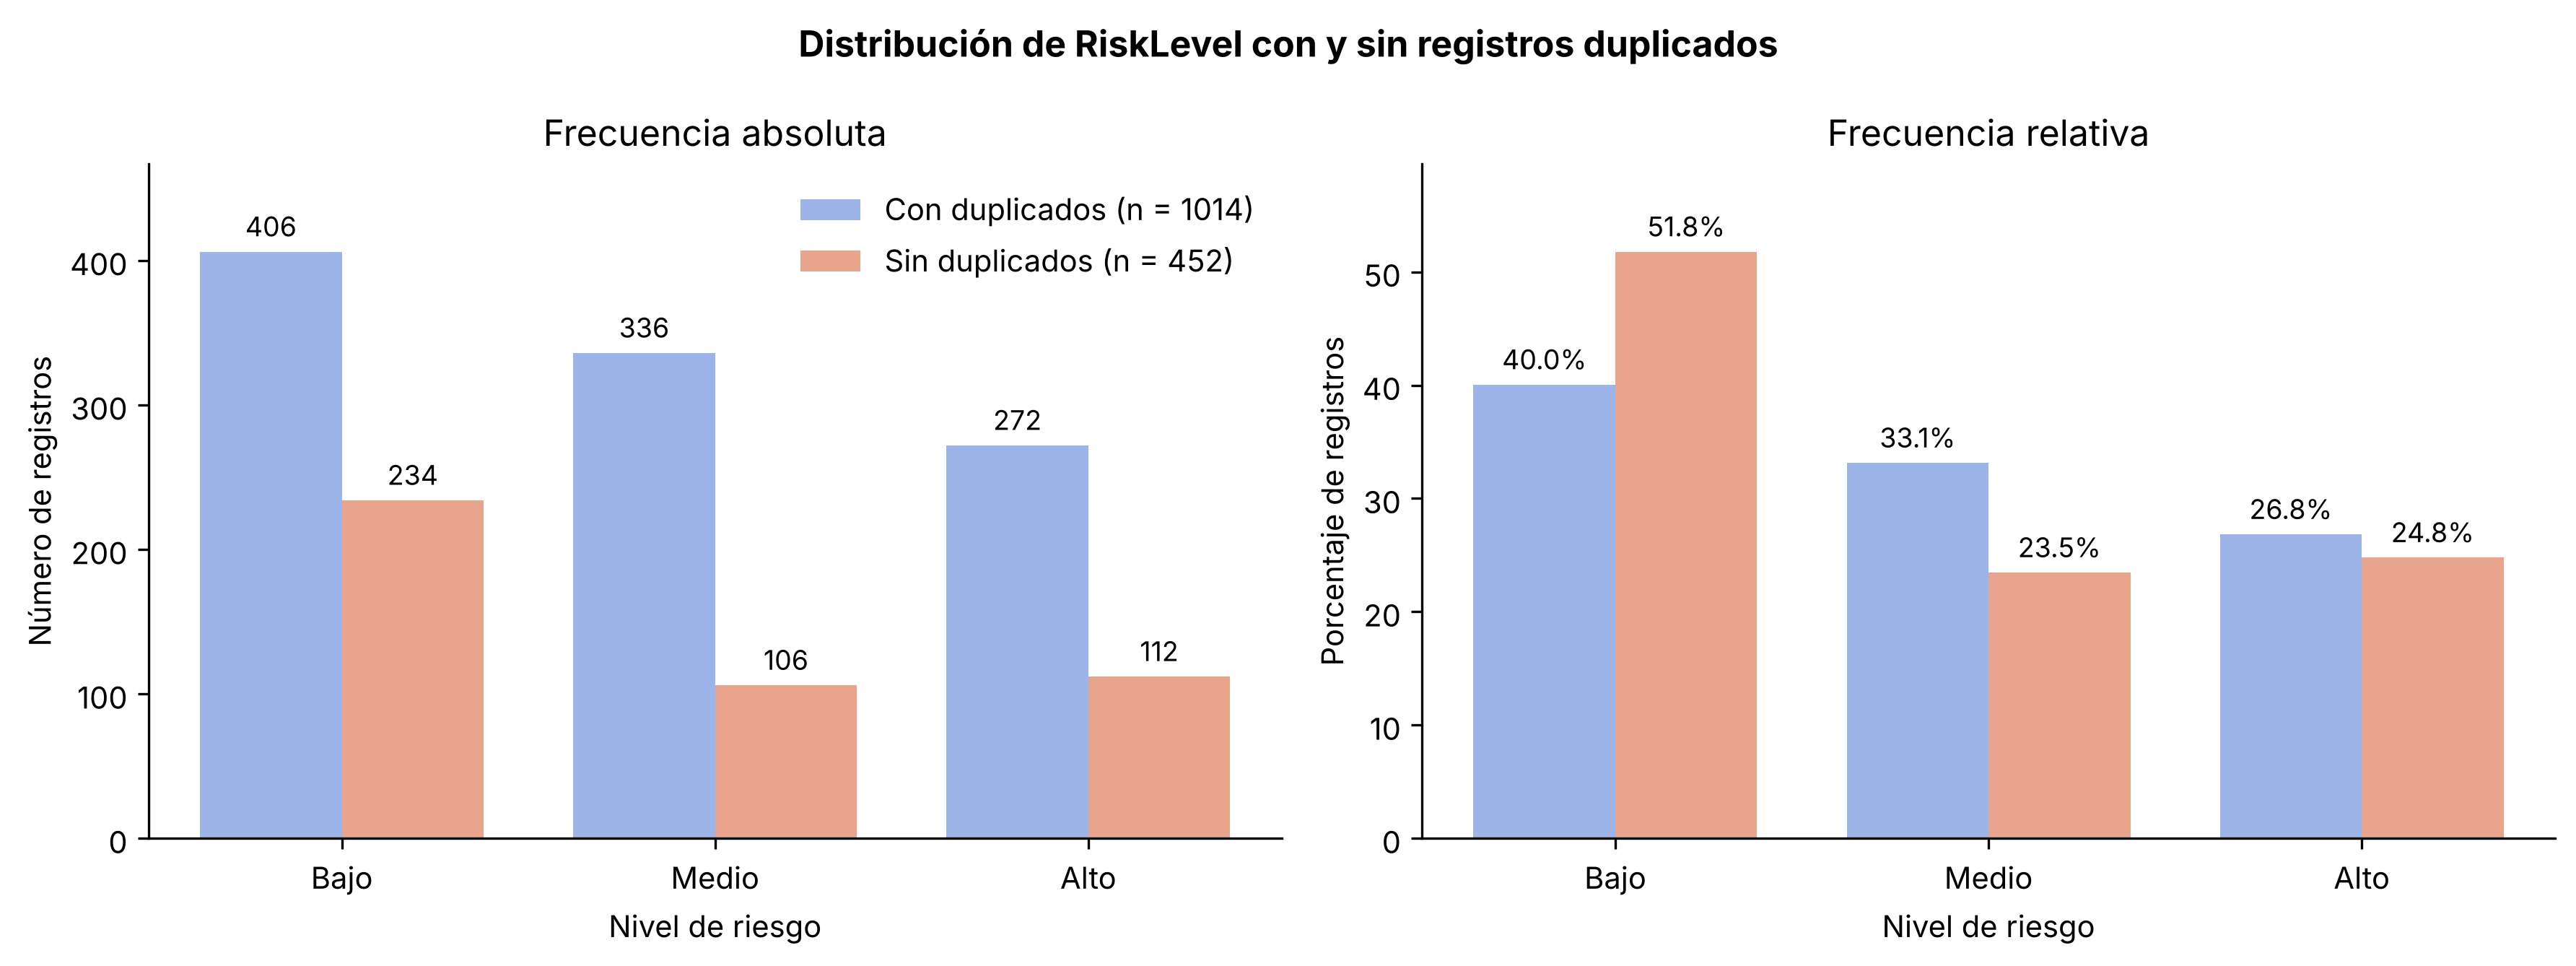
\includegraphics[width=\columnwidth]{eda_clases_duplicados.png}
\caption{Distribución del nivel de riesgo con y sin registros duplicados.}
\label{fig:clases}
\end{figure}

En la base inicial, la mayoría de las variables tienen una distribución unimodal
con colas largas hacia los valores altos, propias de los casos clínicos severos
(Figura~\ref{fig:histogramas}).

\begin{figure*}[t]
\centering
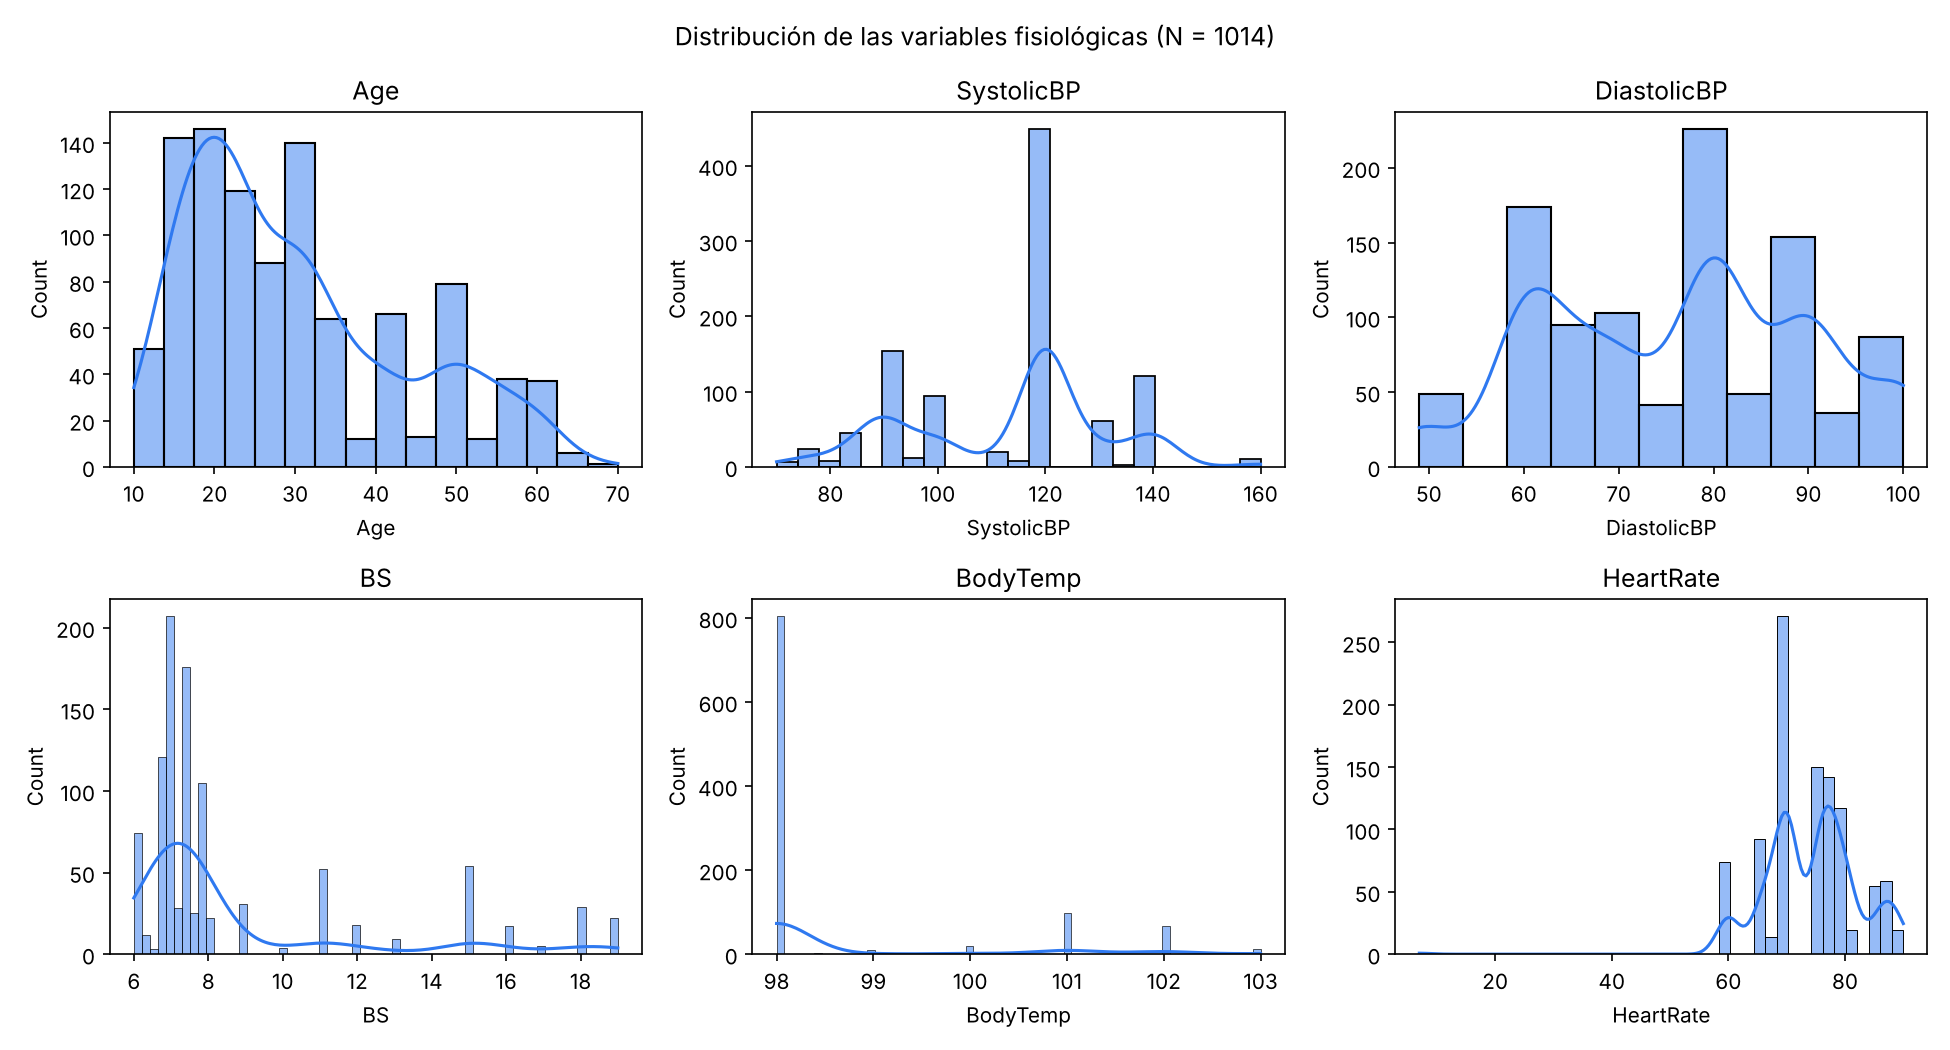
\includegraphics[width=0.85\textwidth]{eda_histogramas_con_duplicados.png}
\caption{Distribución de las variables fisiológicas en la base inicial ($N=1.014$).}
\label{fig:histogramas}
\end{figure*}

La comparación por nivel de riesgo con los registros únicos
(Figura~\ref{fig:boxplots}) muestra que las tres clases se solapan en todas las
variables. La clase de riesgo alto es la más fácil de distinguir, sobre todo por
la glucosa (mediana de 11,0 mmol/L frente a 7,2 y 7,0 en riesgo bajo y medio) y por
la edad (33,5 años frente a 22 y 25,5). Las clases de riesgo bajo y medio son las
más difíciles de separar.

\begin{figure*}[t]
\centering
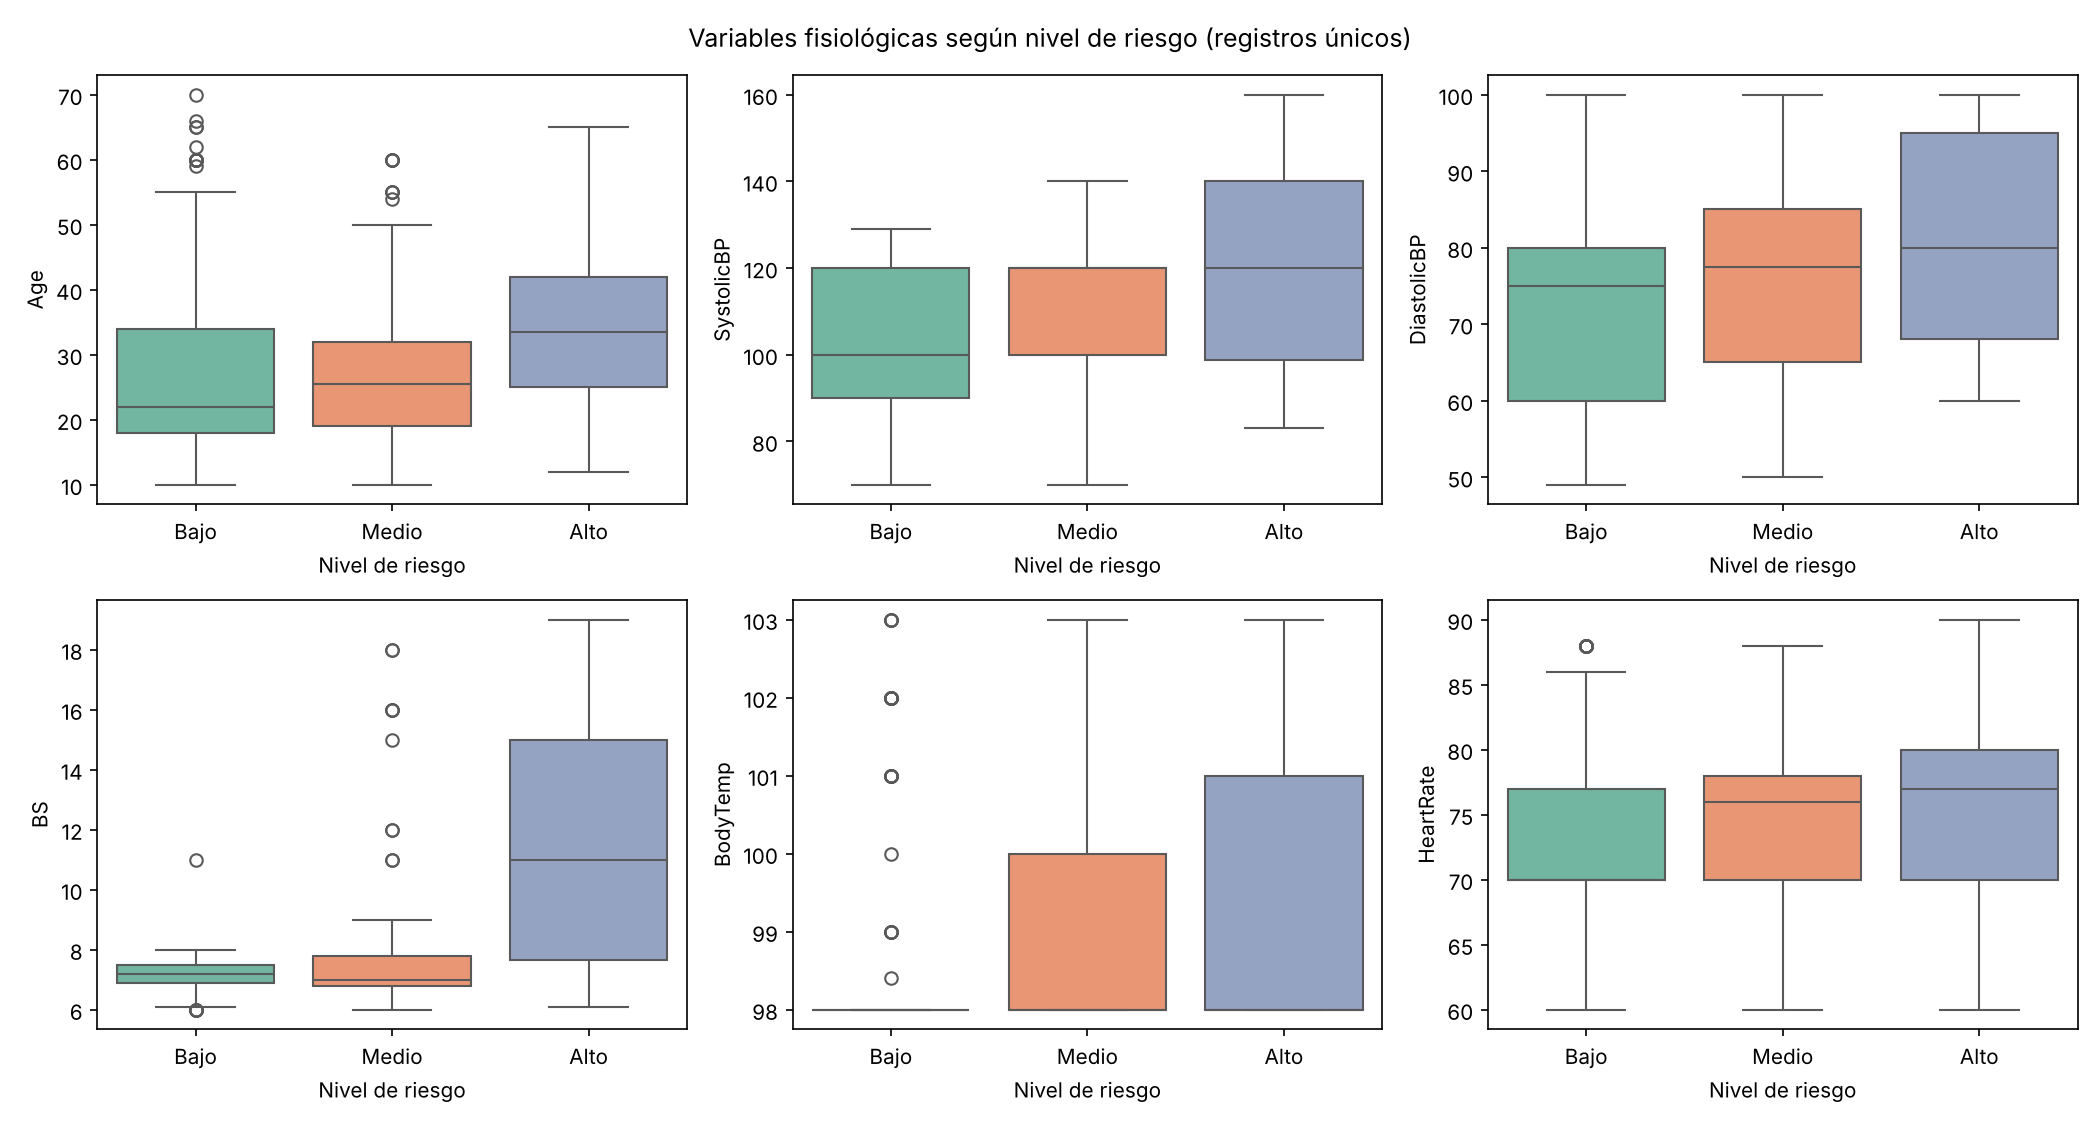
\includegraphics[width=0.85\textwidth]{eda_boxplots_por_riesgo_sin_duplicados.png}
\caption{Variables fisiológicas según el nivel de riesgo (registros únicos, $n=451$).}
\label{fig:boxplots}
\end{figure*}

En la matriz de correlación de la base inicial (Figura~\ref{fig:correlaciones}),
la glucosa es la variable más asociada con el nivel de riesgo ($r=0.57$), seguida
de la presión sistólica ($0.40$) y la diastólica ($0.35$); la temperatura ($0.16$) y
la frecuencia cardíaca ($0.19$) tienen asociaciones bajas. Las dos presiones están
muy correlacionadas entre sí ($r=0.79$), lo que puede dificultar separar sus
efectos en el modelo. Con los registros únicos la glucosa sigue siendo la variable
más asociada ($0.55$), pero las correlaciones de la presión diastólica ($0.25$) y
la edad ($0.18$) bajan, lo que indica que las repeticiones inflaban su aparente
relación con el riesgo.

\begin{figure*}[t]
\centering
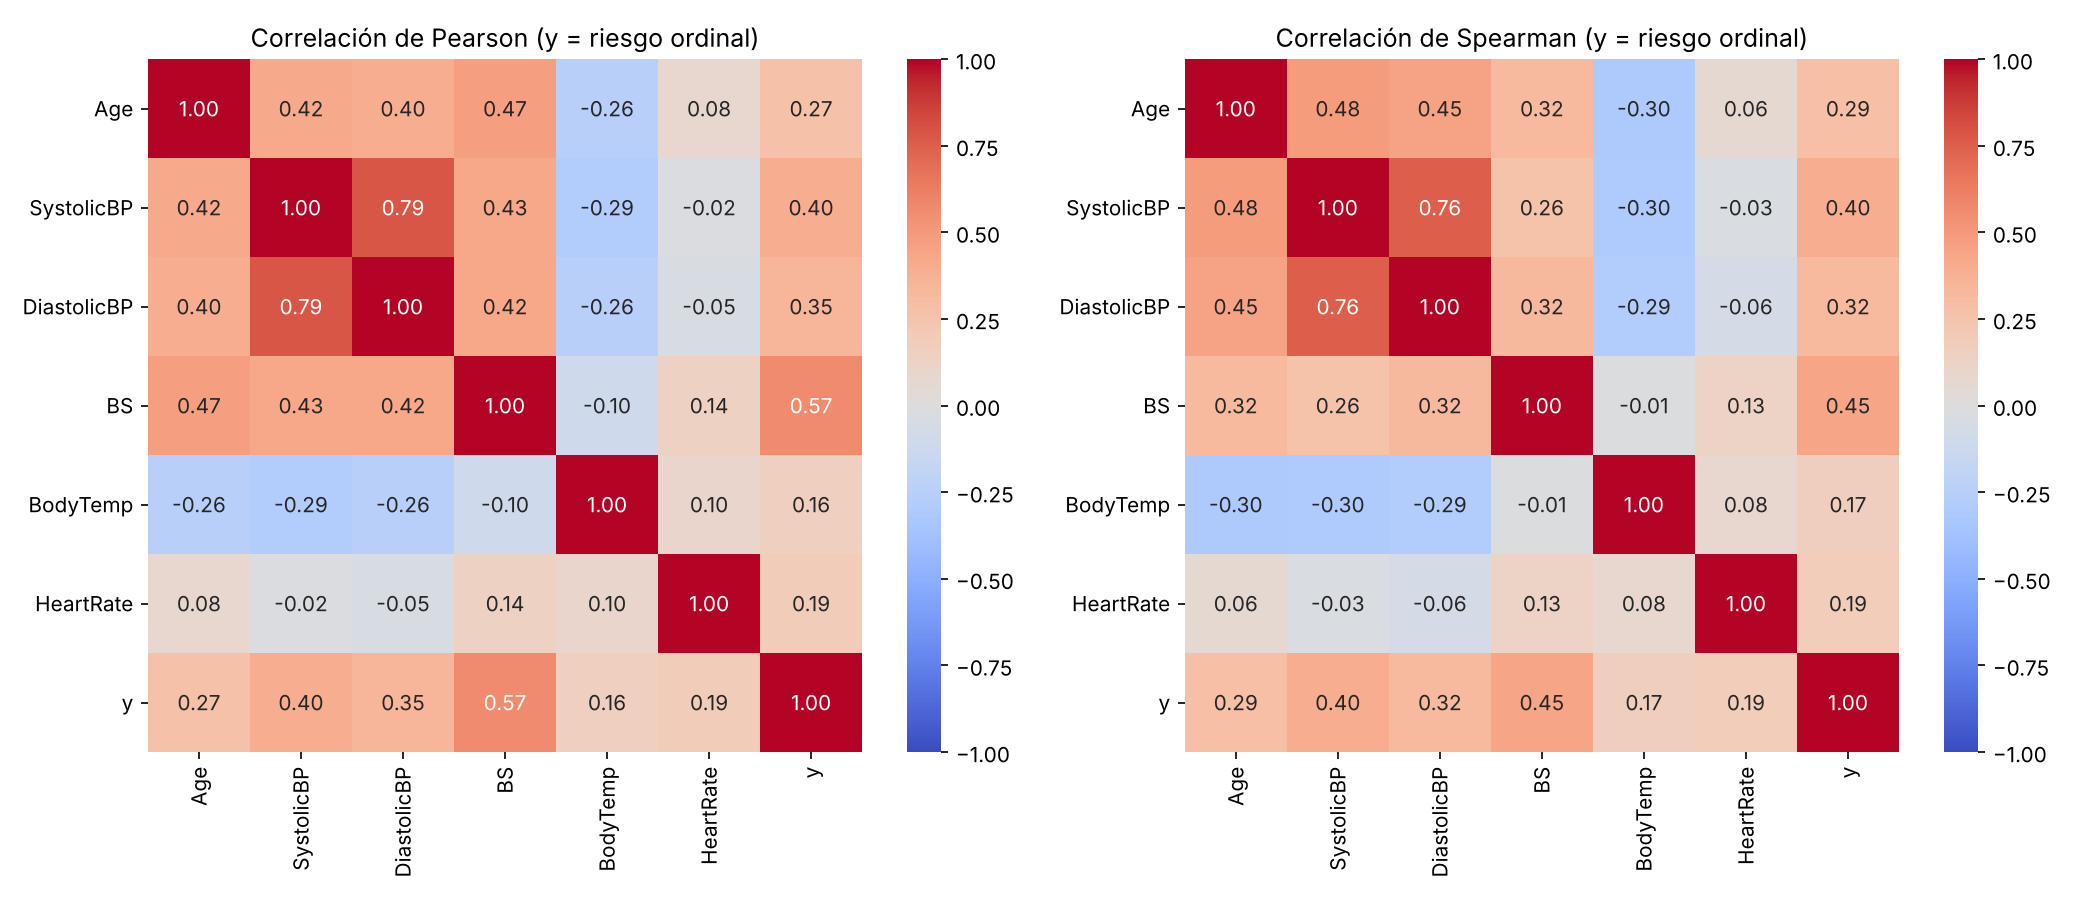
\includegraphics[width=0.85\textwidth]{eda_correlaciones_con_duplicados.png}
\caption{Correlaciones de Pearson y Spearman entre las variables y el nivel de riesgo (base inicial).}
\label{fig:correlaciones}
\end{figure*}
            % A
% Responsable: B
\section{Metodología: inferencia bayesiana}
\subsection{Justificación del modelo}
% TODO
\subsection{Distribución likelihood}
% TODO
\subsection{Especificación de las priors}
% TODO: distribución, hiperparámetros y argumento de cada una.
\subsection{Distribución posterior}
% TODO
     % B
% Responsable: C
\section{Metodología: modelación bayesiana}
\subsection{Algoritmo}
% TODO: Metropolis-Hastings o Gibbs con su pseudocódigo.
\subsection{Implementación del MCMC}
% TODO
     % C
% 
\section{Resultados y discusión}
\subsection{Convergencia}
Para revisar la convergencia se usaron las trazas de cada parámetro, la
autocorrelación, la media acumulada por cadena y dos diagnósticos numéricos: el
$\hat{R}$, que compara la variación entre cadenas con la variación dentro de
cada una, y el tamaño de muestra efectivo (ESS). Se tomaron como criterios
$\hat{R}\leq1.01$ y un ESS de al menos 400 en todos los parámetros.

En la base sin duplicados todos los parámetros cumplen ambos criterios
(Tabla~\ref{tab:convergencia}): el $\hat{R}$ está entre $1.00$ y $1.01$ y el ESS
\emph{bulk} va de 1.003 (BS) a 2.195 (HeartRate), con un ESS de colas mínimo de
1.827. En la base con duplicados ocurre lo mismo, con un ESS \emph{bulk} mínimo
de 871, también para BS. Las cuatro cadenas se superponen en las trazas y la
media acumulada de cada una se estabiliza después del \emph{burn-in} en valores
muy cercanos entre cadenas (Figura~\ref{fig:media_acumulada}); las pequeñas
diferencias que se ven en la edad y la frecuencia cardíaca son mínimas frente a
la desviación de su posterior. Por esto se concluye que las cadenas convergen y
que el número de muestras es suficiente para resumir la posterior.

\begin{table}[h]
\centering
\caption{Diagnósticos de convergencia por parámetro.}
\label{tab:convergencia}
\small
\begin{tabular}{lcccc}
\toprule
 & \multicolumn{2}{c}{Sin duplicados} & \multicolumn{2}{c}{Con duplicados}\\
\cmidrule(lr){2-3}\cmidrule(lr){4-5}
Parámetro & $\hat{R}$ & ESS & $\hat{R}$ & ESS\\
\midrule
$\alpha_1$  & 1.00 & 1366 & 1.01 & 1091\\
$\alpha_2$  & 1.01 & 1282 & 1.00 & 1035\\
Age         & 1.00 & 1809 & 1.00 & 1520\\
SystolicBP  & 1.01 & 1197 & 1.00 & 1233\\
DiastolicBP & 1.00 & 2035 & 1.00 & 1843\\
BS          & 1.00 & 1003 & 1.00 & 871\\
BodyTemp    & 1.00 & 1681 & 1.00 & 1626\\
HeartRate   & 1.00 & 2195 & 1.00 & 2123\\
\bottomrule
\end{tabular}
\end{table}

\begin{figure*}[t]
\centering
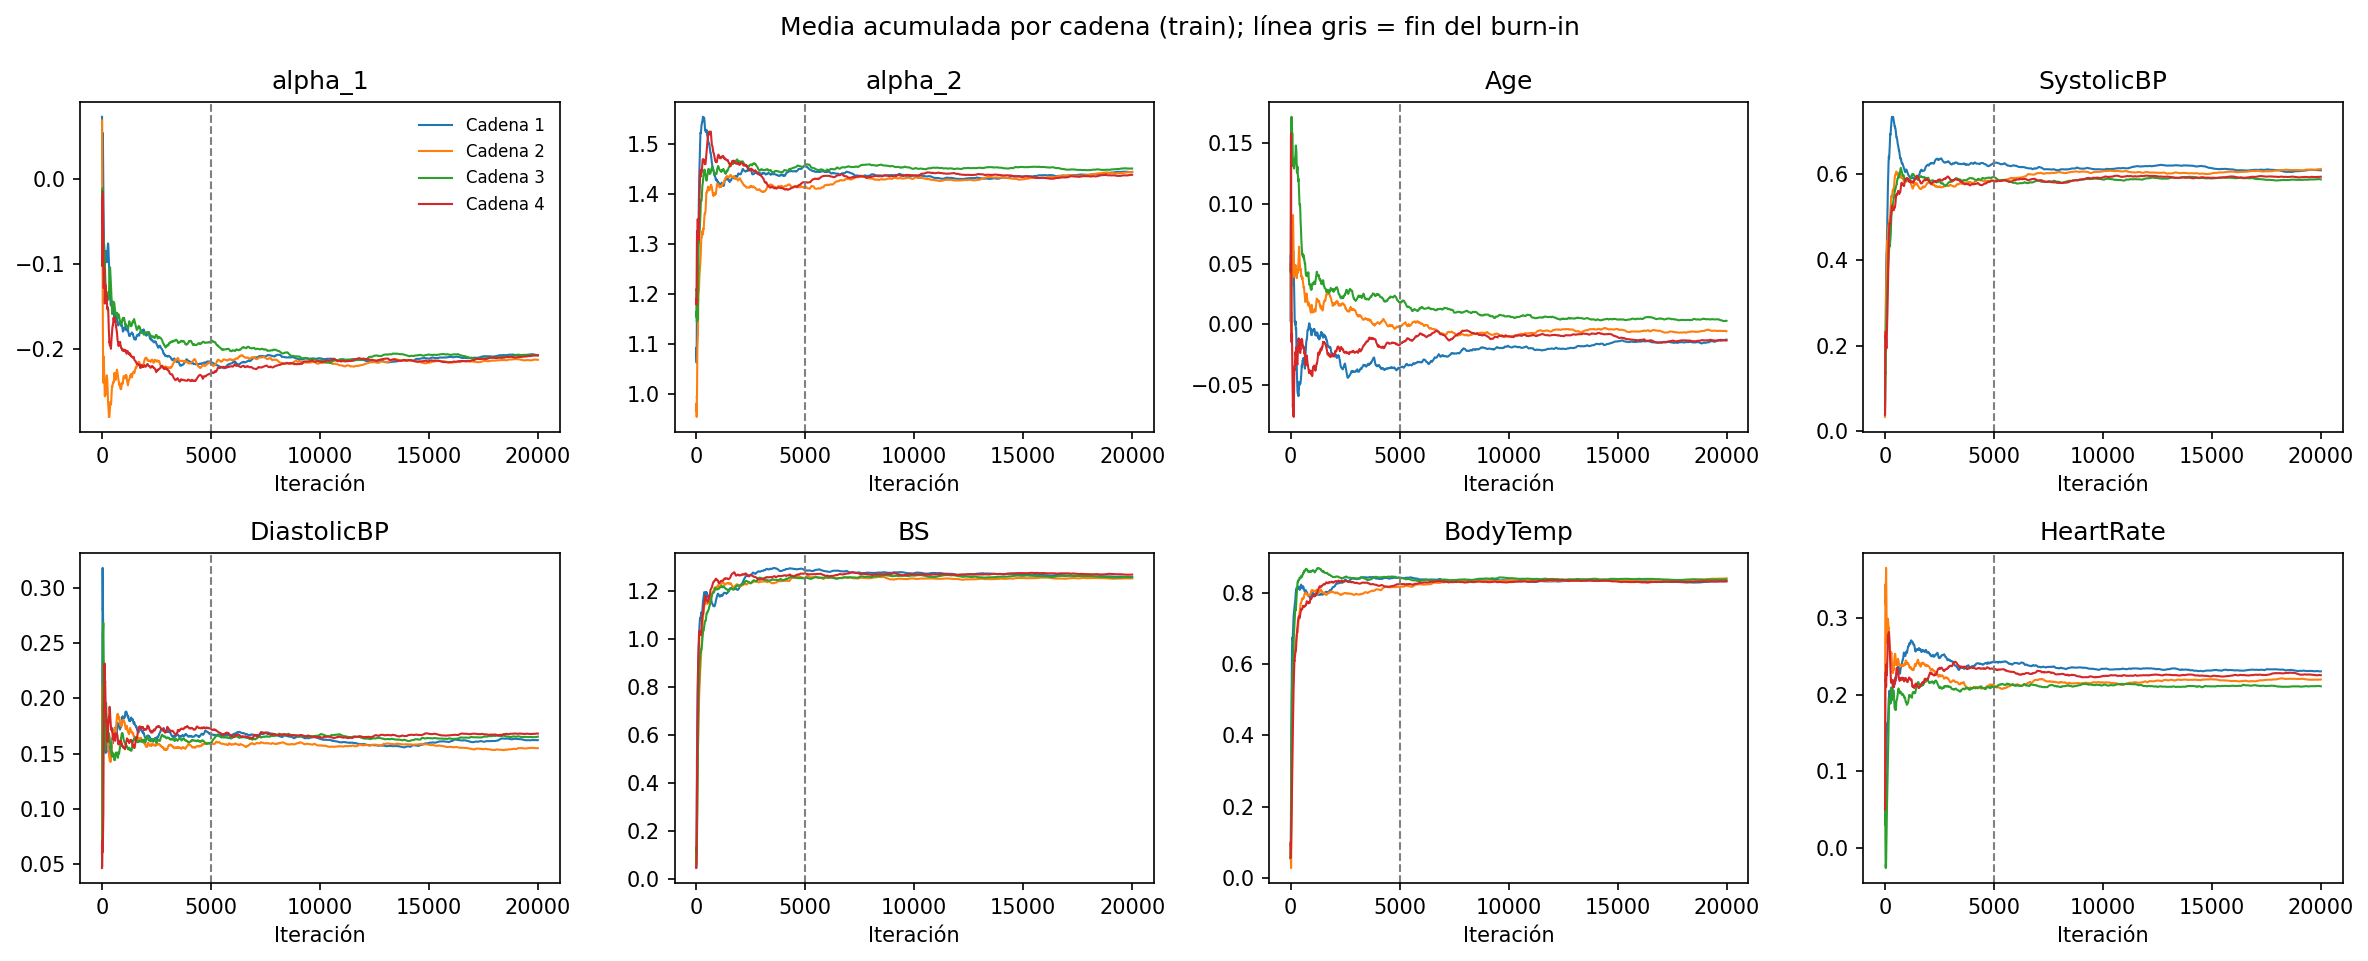
\includegraphics[width=\textwidth]{conv_media_acumulada_train.png}
\caption{Media acumulada de cada parámetro por cadena (base sin duplicados). La línea gris marca el fin del \emph{burn-in}.}
\label{fig:media_acumulada}
\end{figure*}

La comparación entre prior y posterior (Figura~\ref{fig:prior_posterior})
muestra que, para la mayoría de parámetros, la posterior es mucho más angosta
que la prior, es decir, los datos dominan el resultado. Hay dos casos que vale
la pena señalar. En la edad, la prior estaba centrada cerca de $0.4$, pero la
posterior queda alrededor de cero, de modo que los datos contradicen lo que se
esperaba. En la presión diastólica, la posterior se acumula cerca de cero, que
es el límite de su prior truncada.

\begin{figure*}[t]
\centering
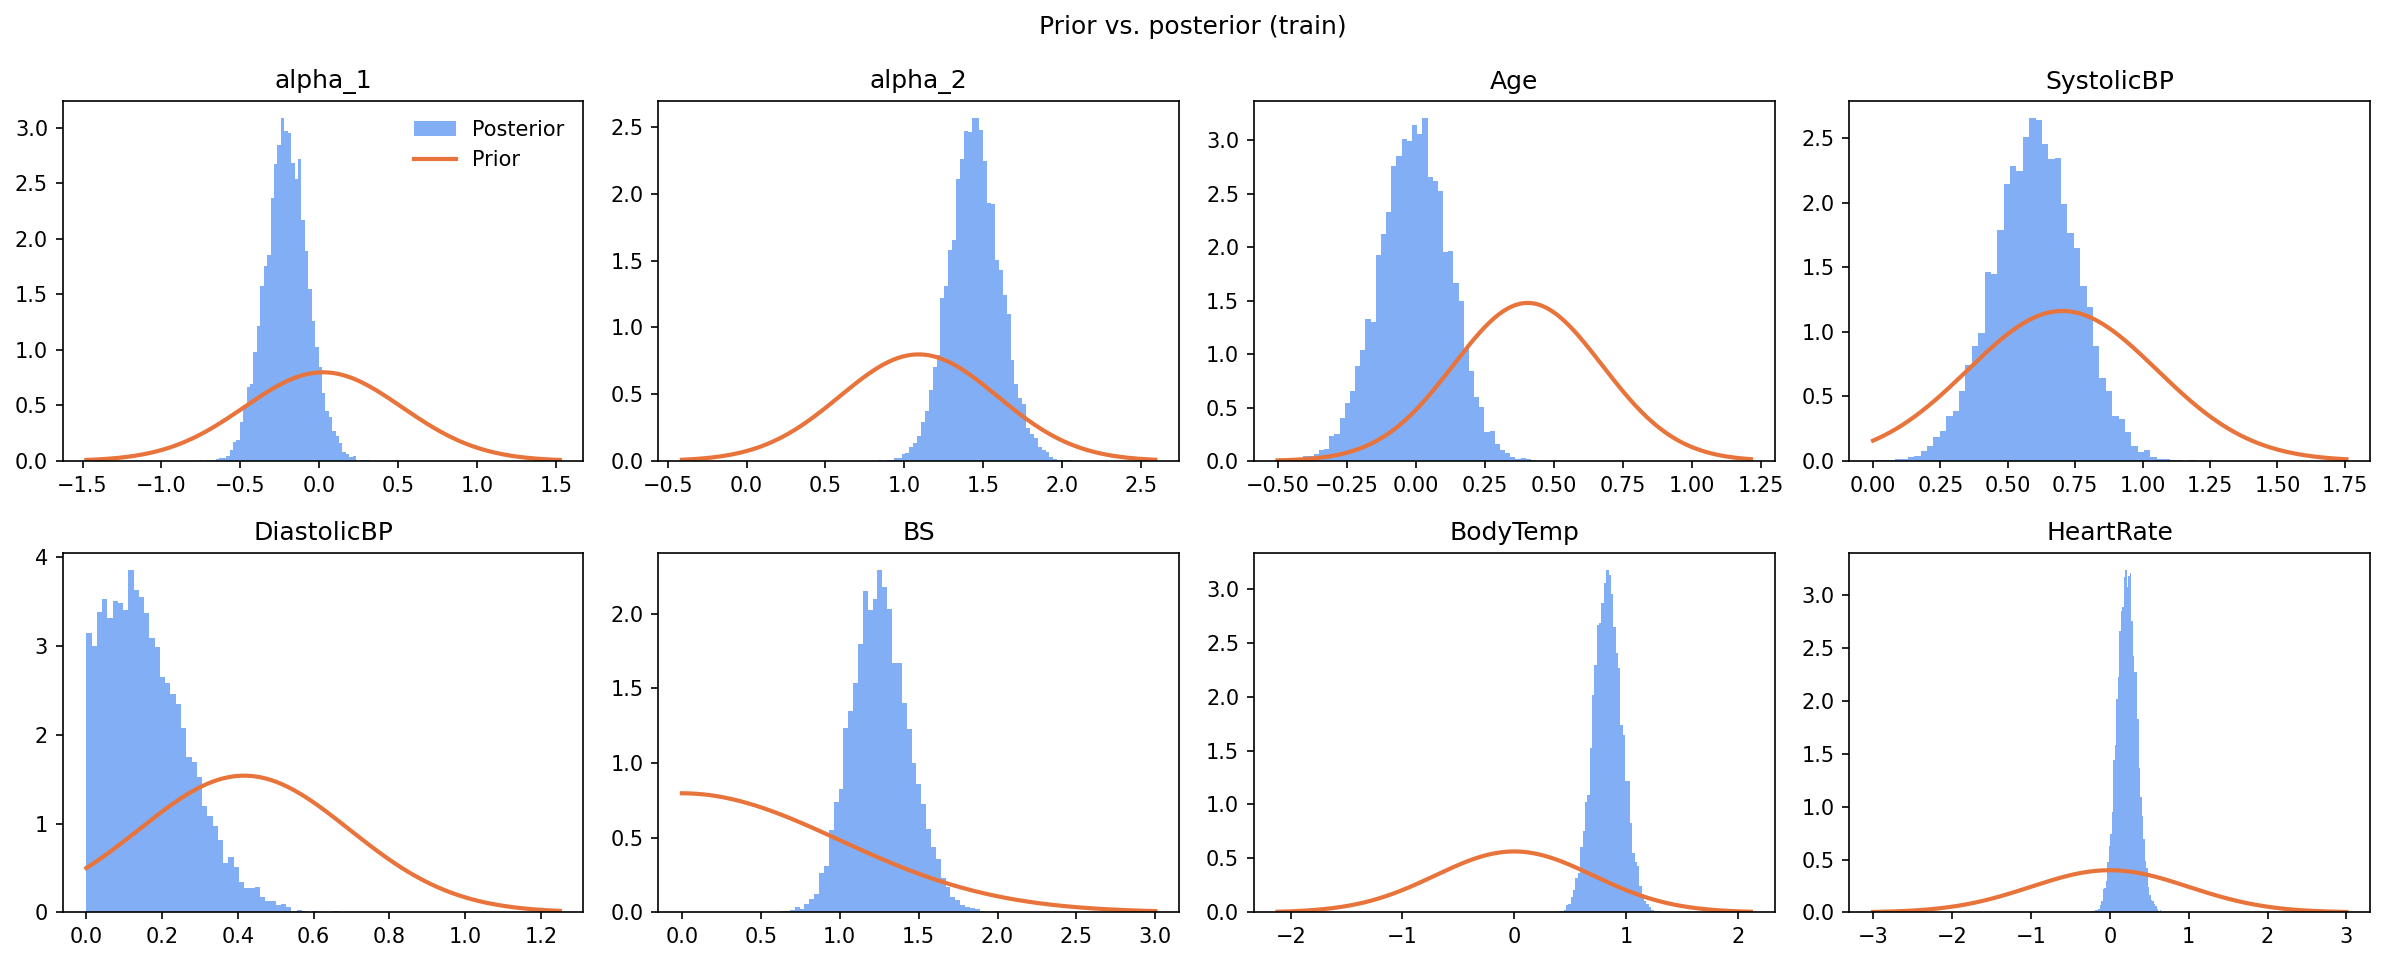
\includegraphics[width=\textwidth]{conv_prior_posterior_train.png}
\caption{Prior (línea) y posterior (histograma) de cada parámetro, base sin duplicados.}
\label{fig:prior_posterior}
\end{figure*}

\begin{table}[h]
\centering
\caption{Resumen de la posterior: media e intervalo de credibilidad del 95\,\%.}
\label{tab:posterior}
\small
\begin{tabular}{lcc}
\toprule
Parámetro & Sin duplicados & Con duplicados\\
\midrule
$\alpha_1$  & $-0.21$ [$-0.47$, $0.07$] & $-0.92$ [$-1.11$, $-0.73$]\\
$\alpha_2$  & $1.45$ [$1.14$, $1.77$]   & $1.23$ [$1.02$, $1.44$]\\
Age         & $-0.01$ [$-0.26$, $0.24$] & $-0.07$ [$-0.25$, $0.11$]\\
SystolicBP  & $0.60$ [$0.29$, $0.90$]   & $0.78$ [$0.56$, $0.99$]\\
DiastolicBP & $0.16$ [$0.01$, $0.41$]   & $0.13$ [$0.01$, $0.31$]\\
BS          & $1.26$ [$0.92$, $1.63$]   & $1.49$ [$1.23$, $1.77$]\\
BodyTemp    & $0.84$ [$0.59$, $1.10$]   & $0.74$ [$0.58$, $0.91$]\\
HeartRate   & $0.22$ [$-0.02$, $0.46$]  & $0.34$ [$0.17$, $0.49$]\\
\bottomrule
\end{tabular}
\end{table}

\subsection{Validación con la base de prueba}
Para cada gestante del conjunto de prueba se calcularon las probabilidades de
las tres clases con cada muestra de la posterior y se promediaron, obteniendo
su probabilidad predictiva. A partir de esas probabilidades se compararon dos
formas de clasificar. La primera es la regla MAP, que asigna la clase más
probable. La segunda es una regla de costo esperado, que asigna la clase con
menor costo según una matriz que sigue el orden de gravedad de los errores
definido en el planteamiento del problema: lo más grave es clasificar como bajo
a una gestante de alto riesgo, le sigue clasificarla como medio, y lo menos
grave es la falsa alarma. La matriz usada, con filas para la clase real y
columnas para la predicha (bajo, medio, alto), es
\[
C=\begin{pmatrix}0&1&2\\2&0&1\\6&3&0\end{pmatrix}.
\]
La incertidumbre de cada métrica se obtuvo calculándola con cada muestra de la
posterior y tomando los percentiles 2.5 y 97.5.

\begin{table}[h]
\centering
\caption{Métricas en la base de prueba sin duplicados ($n=117$).}
\label{tab:metricas}
\small
\begin{tabular}{lcc}
\toprule
Métrica & Costo esperado [IC 95\,\%] & MAP\\
\midrule
Recall alto riesgo  & $0.86$ [$0.75$, $0.93$] & $0.68$\\
Recall riesgo medio & $0.40$ [$0.20$, $0.56$] & $0.04$\\
MCC                 & $0.38$ [$0.30$, $0.41$] & $0.43$\\
Exactitud balanceada& $0.60$ [$0.54$, $0.63$] & $0.55$\\
Exactitud           & $0.59$ [$0.54$, $0.60$] & $0.68$\\
\bottomrule
\end{tabular}
\end{table}

Con la regla MAP el modelo prácticamente no predice la clase de riesgo medio
(recall de $0.04$): las gestantes de esa clase terminan clasificadas como de
riesgo bajo o alto. Esto se debe a que en ninguna gestante la probabilidad de
riesgo medio supera $0.39$, por lo que nunca es la clase más probable. También
se probó una regla que asigna alto riesgo cuando su probabilidad supera un
umbral; con umbrales entre $0.20$ y $0.50$ el recall de alto riesgo va de $0.89$
a $0.68$, pero el de riesgo medio se mantiene entre $0$ y $0.08$, de modo que
mover el umbral no resuelve el problema de la clase media.

La regla de costo esperado sí lo hace, porque usa las tres probabilidades y no
solo la más alta: recupera la clase media (recall de $0.40$) y sube el recall de
alto riesgo de $0.68$ a $0.86$, con la mejor exactitud balanceada ($0.60$). El
precio es un mayor número de falsas alarmas en las gestantes de riesgo bajo, que
es justamente el error que se definió como menos grave, y por eso el MCC y la
exactitud global son algo menores que con la regla MAP (Figura~\ref{fig:confusion}).
Por coherencia con el objetivo del proyecto, que prioriza detectar a las
gestantes de alto riesgo, se toma la regla de costo esperado como regla principal.

\begin{figure}[h]
\centering
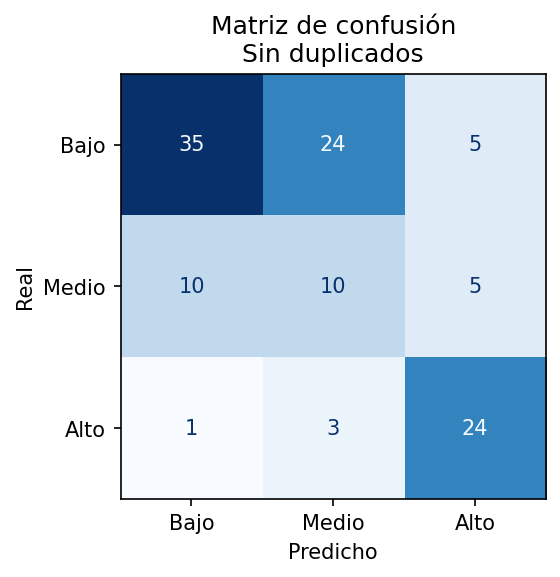
\includegraphics[width=0.49\columnwidth]{eval_confusion_train.png}
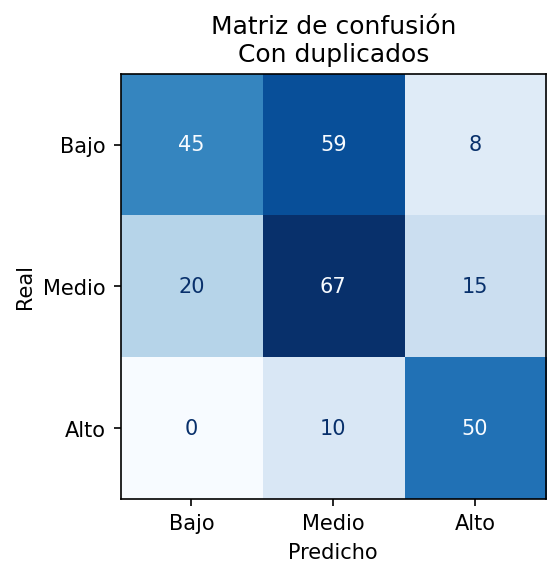
\includegraphics[width=0.49\columnwidth]{eval_confusion_train_full.png}
\caption{Matrices de confusión con la regla de costo esperado: sin duplicados (izq.) y con duplicados (der.).}
\label{fig:confusion}
\end{figure}

\subsection{Respuesta a la pregunta de investigación}
Las variables fisiológicas registradas permiten clasificar el nivel de riesgo de
forma moderada. Con la regla de costo esperado, el modelo detecta 86\,\% de las
gestantes de alto riesgo, con una exactitud balanceada de $0.60$ y un MCC de
$0.38$, pero distingue mal la clase de riesgo medio, que es la más pequeña y la
que más se traslapa con las otras dos.

En cuanto al peso predictivo, y como todas las variables están en la misma
escala, los coeficientes se pueden comparar directamente. La glucemia (BS) es
la variable de mayor peso: un aumento de una desviación estándar multiplica por
cerca de $3.5$ las odds de pasar a un nivel de riesgo mayor. Le siguen la
temperatura corporal ($2.3$) y la presión sistólica ($1.8$), las tres con
intervalos lejos de cero. La frecuencia cardíaca ($1.25$) y la presión
diastólica ($1.18$) tienen un efecto pequeño, y la edad no muestra efecto
($0.99$, con un intervalo centrado en cero).

\subsection{Discusión}
Al comparar con la base con duplicados, el orden de importancia de las variables
se mantiene, con BS, la presión sistólica y la temperatura como las de mayor
peso, y la edad sin efecto. Lo que cambia es la incertidumbre: con duplicados
los intervalos de credibilidad son más angostos, porque cada copia cuenta como
una observación nueva en la likelihood y la posterior parece más precisa de lo
que realmente es. Los puntos de corte también cambian, ya que las proporciones
de las clases son distintas en esa base. En la validación, el recall de alto
riesgo es parecido en ambas ($0.86$ frente a $0.83$), por lo que tener más filas
repetidas no mejora la detección de los casos más graves; además, en la base
con duplicados el conjunto de prueba también repite registros, lo que hace que
sus métricas no sean directamente comparables. Esto respalda la decisión de
trabajar con los registros únicos.

Entre las limitaciones, la principal es la clase de riesgo medio. El modelo
asume odds proporcionales, es decir, un mismo efecto de cada variable en los
dos puntos de corte, y la dificultad para separar esa clase sugiere que este
supuesto no se cumple del todo con estos datos. El resultado de la edad apunta
en la misma dirección: el riesgo aumenta tanto en edades muy bajas como muy
altas, y una relación lineal no capta ese comportamiento. Por otro lado, la
matriz de costos es una decisión del grupo basada en el orden de gravedad de los
errores, no un valor clínico validado, y el conjunto de prueba es pequeño (117
registros), lo que explica la amplitud de algunos intervalos. Finalmente, la
fuente no documenta cómo se asignó la etiqueta de riesgo, por lo que el modelo
aprende a reproducir esa etiqueta y no necesariamente un criterio clínico.
     % C
% Responsables: A, B y C
\section{Conclusiones}

El modelo se estimó con 451 registros únicos y solo seis signos fisiológicos, y
con ellos detectó el 86\,\% de las gestantes de alto riesgo en la base de prueba.
Esto indica que una muestra moderada y un conjunto mínimo de variables medibles
en un puesto rural bastan para sostener una alerta de alto riesgo, aunque no para
graduar los tres niveles. Esto teniendo en cuenta que se tomó la decisión de
eliminar duplicados debido a que al mantenerlos el único efecto era
sobreestimación en las posteriors.

Las estimaciones son confiables desde el punto de vista computacional. Las cuatro
cadenas de Metropolis-Hastings convergieron, con $\hat{R}\leq1.01$ y un ESS mínimo
de 1.003 (glucosa), y las posteriores resultaron mucho más angostas que las
priors. Esto indica que los resultados están determinados por los datos.

En cuanto a las variables, la glucemia fue la de mayor peso ($\mathrm{OR}=3.5$ por
desviación estándar), lo que confirma la hipótesis derivada del análisis
exploratorio, donde ya presentaba la mayor correlación con el riesgo ($r=0.57$).
La presión sistólica ($\mathrm{OR}=1.8$) también confirmó el efecto positivo
esperado a partir de la literatura sobre trastornos hipertensivos. La temperatura
($\mathrm{OR}=2.3$), en cambio, contradijo lo previsto: su prior se centró en cero
por su baja variabilidad, pero ocupó el segundo lugar. Dado que casi todos los
registros se concentran en 98\,°F, este efecto refleja principalmente la presencia
o ausencia de fiebre, se presume que va relacionado con variables que no están
explícitas en el dataset y por lo mismo su explicación puede deberse a relación
con ellas. Además, como se mencionó anteriormente, el modelo es mejor separando
la clase alta y coincide con que los registros con fiebre tienen como etiqueta
riesgo alto.

La regla de decisión determinó buena parte del desempeño. Con la regla MAP, la
clase media casi no se predijo (recall de $0.04$) porque su probabilidad nunca
superó $0.39$, y ajustar un umbral para el alto riesgo tampoco la recuperó: el
recall medio no pasó de $0.08$. La regla de costo esperado elevó el recall de alto
riesgo de $0.68$ a $0.86$, recuperó la clase media hasta $0.40$ y obtuvo la mayor
exactitud balanceada ($0.60$), a cambio de un MCC algo menor ($0.38$ frente a
$0.43$). Esa pérdida proviene del aumento de falsas alarmas, que es el error
definido como menos grave. Se prefirió así un modelo que remite de más a uno que
omite casos graves.

Esta preferencia se justifica por el costo operativo de cada error. Clasificar
como bajo riesgo a una gestante de alto riesgo, el error con mayor peso en la
matriz, implica que no se la remite ni se refuerza su seguimiento, con una
consecuencia potencialmente irreversible. Clasificar como medio a una gestante de
bajo riesgo genera controles adicionales y gastos de transporte, un costo
relevante en un entorno de recursos limitados pero recuperable. Con todo, los
pesos de la matriz son una decisión del grupo y requieren validación clínica.

El bajo desempeño en la clase media sugiere que el supuesto de odds
proporcionales no se cumple del todo: un mismo efecto por variable en ambos
puntos de corte favorece la transición hacia el alto riesgo y deja sin definición
la clase intermedia. Sin embargo, hace parte del trabajo futuro realizar
comparaciones profundas y con otra perspectiva académica.

Además, como la fuente no documenta cómo se asignó RiskLevel, el modelo reproduce
esa etiqueta y no necesariamente un criterio clínico. Si la etiqueta se construyó
con estos mismos signos, parte del desempeño reflejaría la regla de etiquetado.

Por último, la validación externa exige prudencia. Los puntos de corte dependen
de la proporción de clases de esta base, los sensores redondean las mediciones y
la base de prueba es pequeña (117 registros). Aplicar el modelo en otra población
requeriría recalibrarlo y validarlo con datos locales.

El modelo sirve, por tanto, como alerta de alto riesgo que apoya la decisión del
profesional, pero no para graduar el riesgo intermedio. Su mejora depende de una
etiqueta documentada, de modelos que relajen el supuesto de odds proporcionales y
de validación en la población de destino.
   % Todos
\bibliographystyle{apalike}
\bibliography{Bibliografia}
\onecolumn
\appendix
% Responsable: B
\section{Apéndice matemático}
% TODO
       % B
\end{document}
